\documentclass[8pt,a4paper]{article}

\usepackage{atbegshi}
\AtBeginShipoutFirst{\special{pdf:tounicode EUC-UCS2}}


%空白の設定
\usepackage{geometry}
\geometry{left=20truemm, right=20truemm, top=15truemm, bottom=20truemm}


%行間の設定
\renewcommand{\baselinestretch}{1.1}

\makeatletter
\newcommand{\figcaption}[1]{\def\@captype{figure}\caption{#1}}
\newcommand{\tblcaption}[1]{\def\@captype{table}\caption{#1}}
\makeatother
%コマンドの定義
\newcommand{\pcl}{\partial}
\newcommand{\bsm}{\boldsymbol}
\newcommand{\bm}{\boldsymbol}
\newcommand{\tr}{\mathrm{tr}}
\newcommand{\udl}{\underline}

\usepackage[nottoc]{tocbibind} 
\usepackage{booktabs}
\usepackage[dvipdfmx]{graphicx}
\usepackage[dvipdfmx]{color}
\usepackage{amsmath, amssymb}
\usepackage{txfonts}
\usepackage{wrapfig}
\usepackage{ascmac}
\usepackage{booktabs}
\usepackage{tabularx}
\usepackage{url}
\usepackage{color}
\usepackage{scalerel}
\usepackage{subfigure}
\usepackage{listings,jlisting}
\usepackage{comment}
\usepackage{tabularx}
\usepackage{longtable}
\usepackage{here}
\lstset{ 
basicstyle=\ttfamily\scriptsize,
  commentstyle=\textit,
  classoffset=1,
  keywordstyle=\bfseries,
  frame=tRBl,
  framesep=5pt,
  showstringspaces=false,
  numbers=left,
  stepnumber=1,
  numberstyle=\tiny,
  tabsize=2
}

\DeclareMathOperator*{\assem}{\scalerel*{\textsf{A}}{\sum}}
%\usepackage[refeq, refpage, japanese]{nomencl}
%\makenomenclature

\setcounter{tocdepth}{4}
\setcounter{secnumdepth}{3}
\newcommand{\todayd}{\the\year/\the\month/\the\day}


\begin{document} 

\begin{center}
	{\Large BBFE mlflowのマニュアル} \\
\end{center}

\tableofcontents

\section{非圧縮性粘性流れの計算}
\subsection{支配方程式}
非圧縮性粘性流れの運動方程式は以下のNavier-Stokes方程式によって記述される。
\begin{equation}
\rho \frac{D\bm{v}}{Dt} = - \nabla p + \mu \nabla^{2} \bm{v} + \bm{f}
\end{equation}
ここで、$\rho$は流体の密度、$\bm{v}$は流体の速度ベクトル、$p$は流体の圧力、$\mu$は流体の粘性係数、$\bm{f}$は外力ベクトルを表す。

また、非圧縮性流れにおける連続の式は以下のように表される。
\begin{equation}
\nabla \cdot v = 0
\end{equation}

本研究では、流体は非圧縮性粘性を仮定しているため、Navier-Stokes方程式(2.9)と非圧縮性の連続の式(2.12)を解く。

\subsection{Fractional step法}

\begin{comment}
本研究の流体解析プログラムでは、流体を解く手法として分離型解法の一つであるFractional Step法を使用した。

式(2.9)のNavier-Stokes方程式において、外力項を省略し、両辺を流体の密度$\rho$で割って無次元化したNavier-Stokes方程式は以下のように記述される。ここではEinsteinの縮約記法を用いる。
\begin{equation}
	\frac{v^{n+1}_i - v^{n}_i}{\Delta t} + v^{n}_i \frac{\partial v^{n}_i}{\partial x_j}
	+ \frac{\partial p^{n+1}}{\partial x_i} - \frac{1}{\mathrm{Re}} \frac{\partial^{2} v^{n}_i}{\partial x^{2}_j} = 0
\end{equation}
ここで$v^{n}_{i}$は$n$ステップ目における$i$方向の流速、$\mathrm{Re}$はレイノルズ数を表す。

また、$n+1$ステップ目を満たす連続の式は以下のように記述される。
\begin{equation}
	\frac{\partial v_{i}^{n+1}}{\partial x_{i}}=0
\end{equation}

式(2.13)の発散を取り、式(2.14)に代入すると以下の圧力Poisson方程式が導かれる。
\begin{equation}
\frac{\partial^2 p^{n+1}}{\partial x^{2}_i} = \frac{1}{\Delta t} \frac{\partial \tilde{v}_i}{\partial x_{i}}
\end{equation}

ここで$\tilde{v}_{i}$は中間流速であり、以下の式で記述される。
\begin{equation}
	\tilde{v}_{i} = v_{i}^{n} - \Delta t
	\left(v_{j}^{n} \frac{\partial v_{i}^{n}}{\partial x_{j}} 
	- \frac{1}{\mathrm{Re}} \frac{\partial^{2} v_{i}^{n}}{\partial x_{j}^{2}}\right)
\end{equation}

圧力Poisson方程式を解いて求めた$n+1$ステップ目の圧力$p^{n+1}$を使って速度を修正することで$n+1$ステップ目の流速$v^{n+1}_{i}$を次式により求める。
\begin{equation}
v^{n+1}_i=\tilde{v}_i - \Delta t \frac{\partial p^{n+1}}{\partial x_i}
\end{equation}
\end{comment}

\subsection{SUPG法による定式化}

\begin{comment}
Navier-Stokes方程式を数値的に解く時、移流項が卓越する場合には数値的な不安定性が生じるという問題がある。
有限要素法において、移流項による数値不安定性を防ぐ方法として、SUPG(Streamline Upwind/Petrov-Galerkin)法が提案された。SUPG法は、移流項の重みを変化させることで、流れの流線方向にのみ安定化させることができる手法である。

Fractional Step法を用いて定式化した式(2.15)・(2.16)・(2.17)にSUPG法を適用する。
Galerkin法に基づいて、流速の重み関数$w_{i}$、流速$v_{i}$、中間流速$\tilde{v}_{i}$、圧力の重み関数$q$、圧力$p$を次のように近似する。
\begin{equation}
	\begin{split}
		w_{i}^{h}=&N_{\alpha}^{e} w_{i\alpha}^{e},\; v_{i}^{h}=N_{\alpha}^{e} v_{i\alpha}^{e},\; 
		\tilde{v}_{i}^{h}=N_{\alpha}^{e} \tilde{v}_{i\alpha}^{e}, \\
		q^{h}=&L_{\alpha}^{e} q_{\alpha}^{e}, \; p^{h}=L_{\alpha}^{e} p_{\alpha}^{e} \\
	\end{split}
\end{equation}
ここで$v_{i\alpha}^{e}$、$\tilde{v}_{i\alpha}^{e}$、$p_{\alpha}$はそれぞれ流速、中間流速、圧力の節点値である。また、$N_{\alpha}$、$L_{\alpha}$はそれぞれ流速場と圧力場に対する形状関数である。$e$は要素のインデックスを表す。

中間流速を求める式は以下の通り。
\begin{equation}
	\begin{split}
		\int_{\Omega} w_{i}\left( \frac{\tilde{v}-v^{n}_i}{\Delta t} + v^{n}_{j} \frac{\partial v^{n}_{i}}{\partial x_{j}}\right) \; d\Omega \;+ 
		\int_{\Omega} \frac{1}{\mathrm{Re}} \frac{\partial w_{i}}{\partial x_{j}} \frac{\partial v^{n}_{i}}{\partial x_{j}} \; d\Omega \;+& \\
		\sum_{e=1}^{M} \int_{\Omega_{e}} \tau_{m} v_{j}^{n} \frac{\partial w_{i}^{h}}{\partial x_{j}} \left( \frac{\tilde{v_{i}} - v_{i}^{n}}{\Delta t} + v_{j}^{n} \frac{\partial v_{i}^{n}}{\partial x_{j}} - \frac{1}{Re} \frac{\partial^{2} v_{i}^{n}}{\partial x_{j}^{2}}\right) \; d\Omega \;=& 
		\int_{\Gamma_{h}} w_{i}\frac{1}{\mathrm{Re}} \frac{\partial v_{i}}{\partial x_{j}}n_{j} \;d\Gamma
	\end{split}
\end{equation}

ここで$e$は要素のインデックス、$M$は全要素数、$\Omega_{e}$は要素領域、$\tau_{m}$は安定化パラメータであり、要素での安定化パラメータ$\tau_{m}^{e}$は次式で与えられる。
\begin{equation}
\tau_{m}^{e}=\left[ \left(\frac{2}{\Delta t}\right)^{2} + \left(\frac{2||\bm{v}||}{h_{e}}\right)^{2} + \left(\frac{4}{\mathrm{Re_{v}} h_{e}^{2}}\right)^{2}\right]^{-1/2}
\end{equation}
$\Delta t$は時間刻み幅、$\bm{v}$は流速、$h_e$は要素サイズ、$\mathrm{Re_u}$は要素レイノルズ数である。

圧力ポアソン方程式は以下のようになる。
\begin{equation}
\int_{\Omega} q \frac{\partial^{2}p^{n+1}}{\partial x_{i}^{2}} \; d\Omega = 
\frac{1}{\Delta t} \int_{\Omega} q \frac{\partial \tilde{v}_{i}}{\partial x_{i}} \; d\Omega
\end{equation}
速度の修正の式は以下のようになる。
\begin{equation}
\int_{\Omega} w_{i}v_{i}^{n+1} \; d\Omega = \int_{\Omega} w_{i} \tilde{v}_{i} \; d\Omega
- \Delta t \int_{\Omega} w_{i} \frac{\partial p^{n+1}}{\partial x_{i}} d\Omega
\end{equation}

式(2.19)・(2.21)・(2.22)を行列で表すとそれぞれ式(2.23)・(2.24)・(2.25)になる。ただし、式(2.21)に対しては部分積分を行う。
\begin{equation}
( \bm{M} + \bm{M}_{s} ) \frac{\tilde{\bm{v}}_i - \bm{v}_{i}^{n}}{\Delta t} + ( \bm{A} + \bm{A}_s ) \bm{v}_{i}^{n} + \bm{D} \bm{v}_{i}^{n} = 0
\end{equation}

\begin{equation}
-\bm{G} \bm{p}^{n+1} = \frac{1}{\Delta t} \bm{C} \tilde{\bm{v}}_{i} - \bm{G}_{\Gamma}
\end{equation}

\begin{equation}
\bm{M} \bm{v}_{i}^{n+1} = \bm{M} \tilde{\bm{v}}_{i} - \Delta t \bm{C} \bm{p}^{n+1}
\end{equation}
\end{comment}

\section{レベルセット法による自由表面流れの計算}
\subsection{支配方程式}
\begin{equation}
	\frac{\partial \phi}{\partial t} + \bm{u} \cdot \nabla \phi = 0 \quad in \quad \Omega
\end{equation}

\subsection{表面張力}
表面張力$\bm{f}_{fs}$とすると、CSF(Continuum Surface Force)モデルにより次式のように算定できる。
\begin{equation}
	\bm{f}_{fs} = \sigma \kappa \nabla \phi
							= \sigma (-\nabla \cdot \frac{\nabla \phi}{|\nabla \phi|}) \nabla \phi
\end{equation}

界面の曲率$\kappa$と法線方向$\bm{n}_{s}$は以下のようにあらわされる。
\begin{equation}
	\bm{n}_{s} = \frac{\nabla \phi}{| \nabla \phi |}
\end{equation}

\begin{equation}
	\kappa = - \nabla \cdot \bm{n}_{s}
\end{equation}



\section{プログラム解説}
\subsection{プログラムの構成}
\begin{itemize}
 \item FE\_solvers
    \begin{itemize}
      \item mlflow\_fs
      	\begin{itemize}
      		\item mlflow\_fs.c
      		\item mlflow\_core.c
      	\end{itemize}
    \end{itemize}
\end{itemize}

\subsection{入力ファイル}
\begin{itemize}
	\item 節点および要素データ: node.dat, elem.dat
	\item 圧力の Dirichlet 境界条件ファイル : D\_bc\_p.dat
	\item 速度の Dirichlet 境界条件ファイル (流入境界条件および noslip 境界条件): D\_bc\_v.dat
	\item レベルセット関数データ:levelset.dat
\end{itemize}

\subsection{出力ファイル}
\begin{itemize}
	\item 結果データ: result\*.vtk
\end{itemize}

\subsection{関数群}
\subsection*{mflow\_fs.c}

void set\_element\_vec\_levelset()

\subsection{実行例}
\subsubsection{入力ファイルの作成}
\begin{lstlisting}[]
#!/bin/bash

cd ./util
mkdir ./workspace/3d-bubble
cd ./workspace/3d-bubble

../../meshgen/meshgen_tet 1.0 1.0 2.0
# -> node.dat と elem.dat を出力
../../surface/surf_conn 1
# -> surf.dat を出力

# 流出境界部の圧力0の境界の切り出し
../../mesh/mesh_surf_extract 0.0 0.0 2.0 1.0 1.0 2.0 -oe surf_p.dat -ov surf_p.vtk
# noslip 境界部の切り出し
../../mesh/mesh_surf_remove 0.0 0.0 2.0 1.0 1.0 2.0 -oe surf_v.dat -ov surf_v.vtk
# 圧力の Dirichlet B.C. ファイルの作成
../../surface/surf_dbc 1 0.0 -ie surf_p.dat -o D_bc_p.dat
# 速度の Dirichlet B.C. ファイル (流入境界および slip 境界) を作成
../../surface/surf_dbc 3 0.0 0.0 0.0 -ie surf_v.dat -o D_bc_v.dat
\end{lstlisting}

\subsubsection{実行}
\begin{lstlisting}[]
#!/bin/bash
cd ../../.../FE_solver/mlflow_fs
mkdir 3d-bubble

./mlflow_fs ./3d-bubble
\end{lstlisting}


\newpage
\section{3次元キャビティ流れ問題}
二層流で二つの流体が同じパラメータの場合に、単層の流れの結果と同じになるかを確認した。

\subsection{解析条件}
\renewcommand{\arraystretch}{1}
\begin{table}[H]
	\centering
	\caption{解析パラメータ}
	\begin{tabular}{cccccc}
		\hline
		Test case & $\rho_1$ & $\rho_2$ & $\mu_1$ & $\mu_2$ & $\mathrm{g}$\\
		\hline 
		Case$1$ & $1$ & $1$ & $0.01$ & $0.01$   & $0$ \\
		\hline         
	\end{tabular}
	\label{table:mars-env}
\end{table}
\renewcommand{\arraystretch}{1.0}

\subsection{解析結果}
\begin{figure}[htbp]
	\centering
	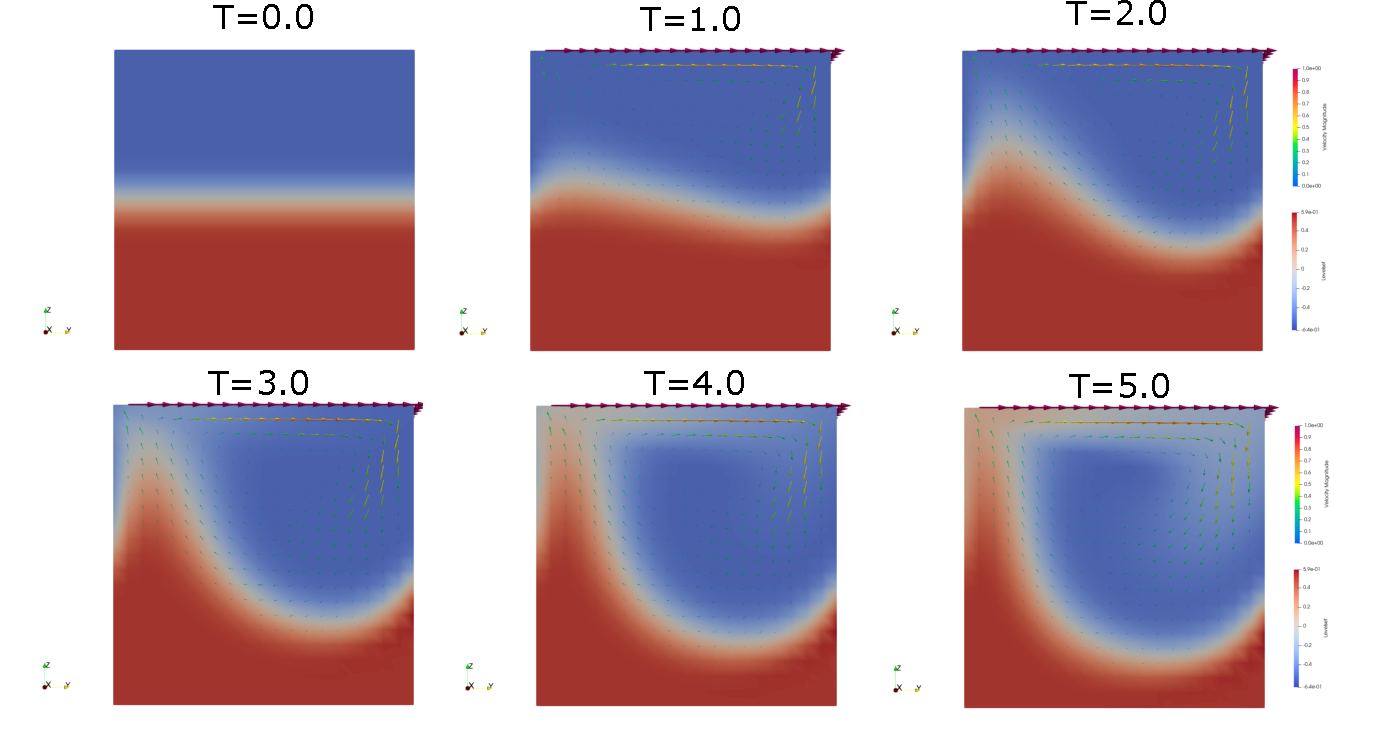
\includegraphics[width=18truecm]{pics/3d-cavity/levelset_velocity.pdf}
	\caption{レベルセット関数}
	\label{fig:3d-bubble-levelset_t0-3}
\end{figure}

\begin{figure}[htbp]
	\centering
	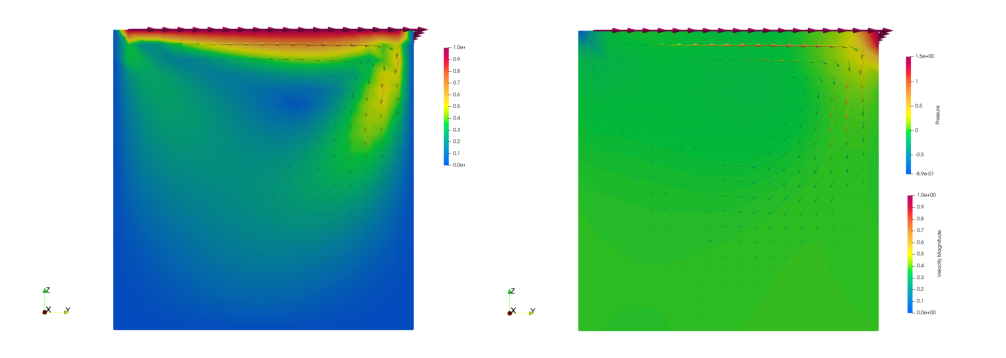
\includegraphics[width=18truecm]{pics/3d-cavity/velocity_pressure.pdf}
	\caption{速度と圧力の結果(二層流れ)}
	\label{fig:3d-bubble-levelset_t0-3}
\end{figure}

\begin{figure}[htbp]
	\centering
	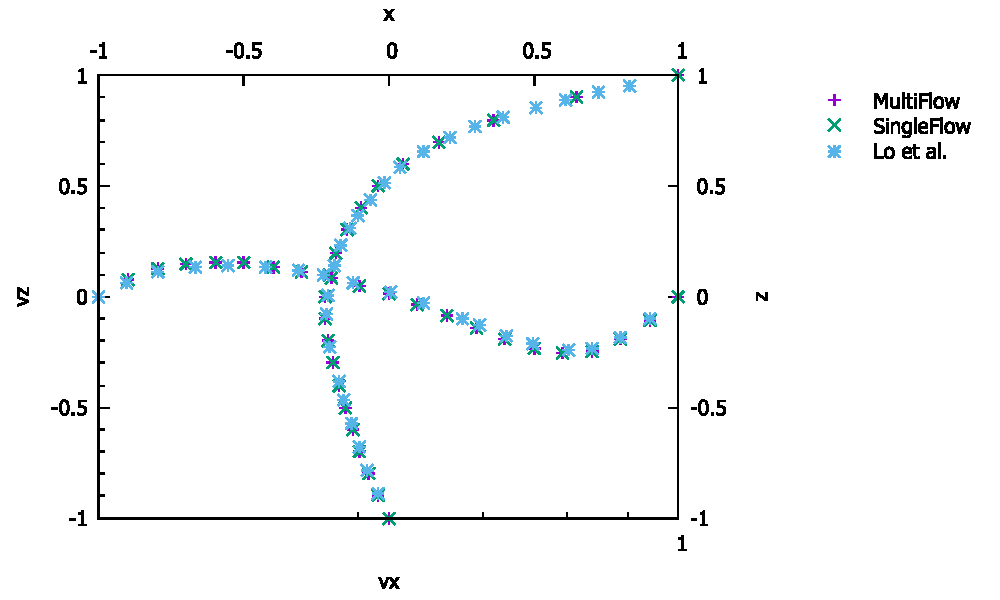
\includegraphics[width=18truecm]{pics/3d-cavity/velocity_graph.pdf}
	\caption{速度分布の検証}
	\label{fig:3d-bubble-levelset_t0-3}
\end{figure}

\newpage
\section{3次元のダムブレイク問題}
\subsection{解析条件}

\renewcommand{\arraystretch}{1}
\begin{table}[H]
	\centering
	\caption{解析パラメータ}
	\begin{tabular}{cccc}
		\hline
		Test case & $\Delta t$ & メッシュ幅$dx$ & ヘビサイド関数パラメータ$D$\\
		\hline 
		Case$1$ & $0.0001$ & $0.05$ & $0.05$\\
		Case$2$ & $0.0001$ & $0.05$ & $0.15$\\
		\hline         
	\end{tabular}
	\label{table:mars-env}
\end{table}
\renewcommand{\arraystretch}{1.0}

\renewcommand{\arraystretch}{1}
\begin{table}[H]
	\centering
	\caption{物性値}
	\begin{tabular}{ccccccc}
		\hline
		Test case & $\rho_1$ & $\rho_2$ & $\mu_1$ & $\mu_2$ & $\mathrm{g}$ \\
		\hline 
		Case$1$ & $1000$ & $1$   & $1\times10^{-3}$ & $1\times10^{-5}$ & $9.81$ \\
		Case$2$ & $1000$ & $100$ & $1\times10^{-3}$ & $1\times10^{-3}$ & $9.81$ \\
		\hline         
	\end{tabular}
	\label{table:mars-env}
\end{table}
\renewcommand{\arraystretch}{1.0}

\begin{figure}[htbp]
	\centering
	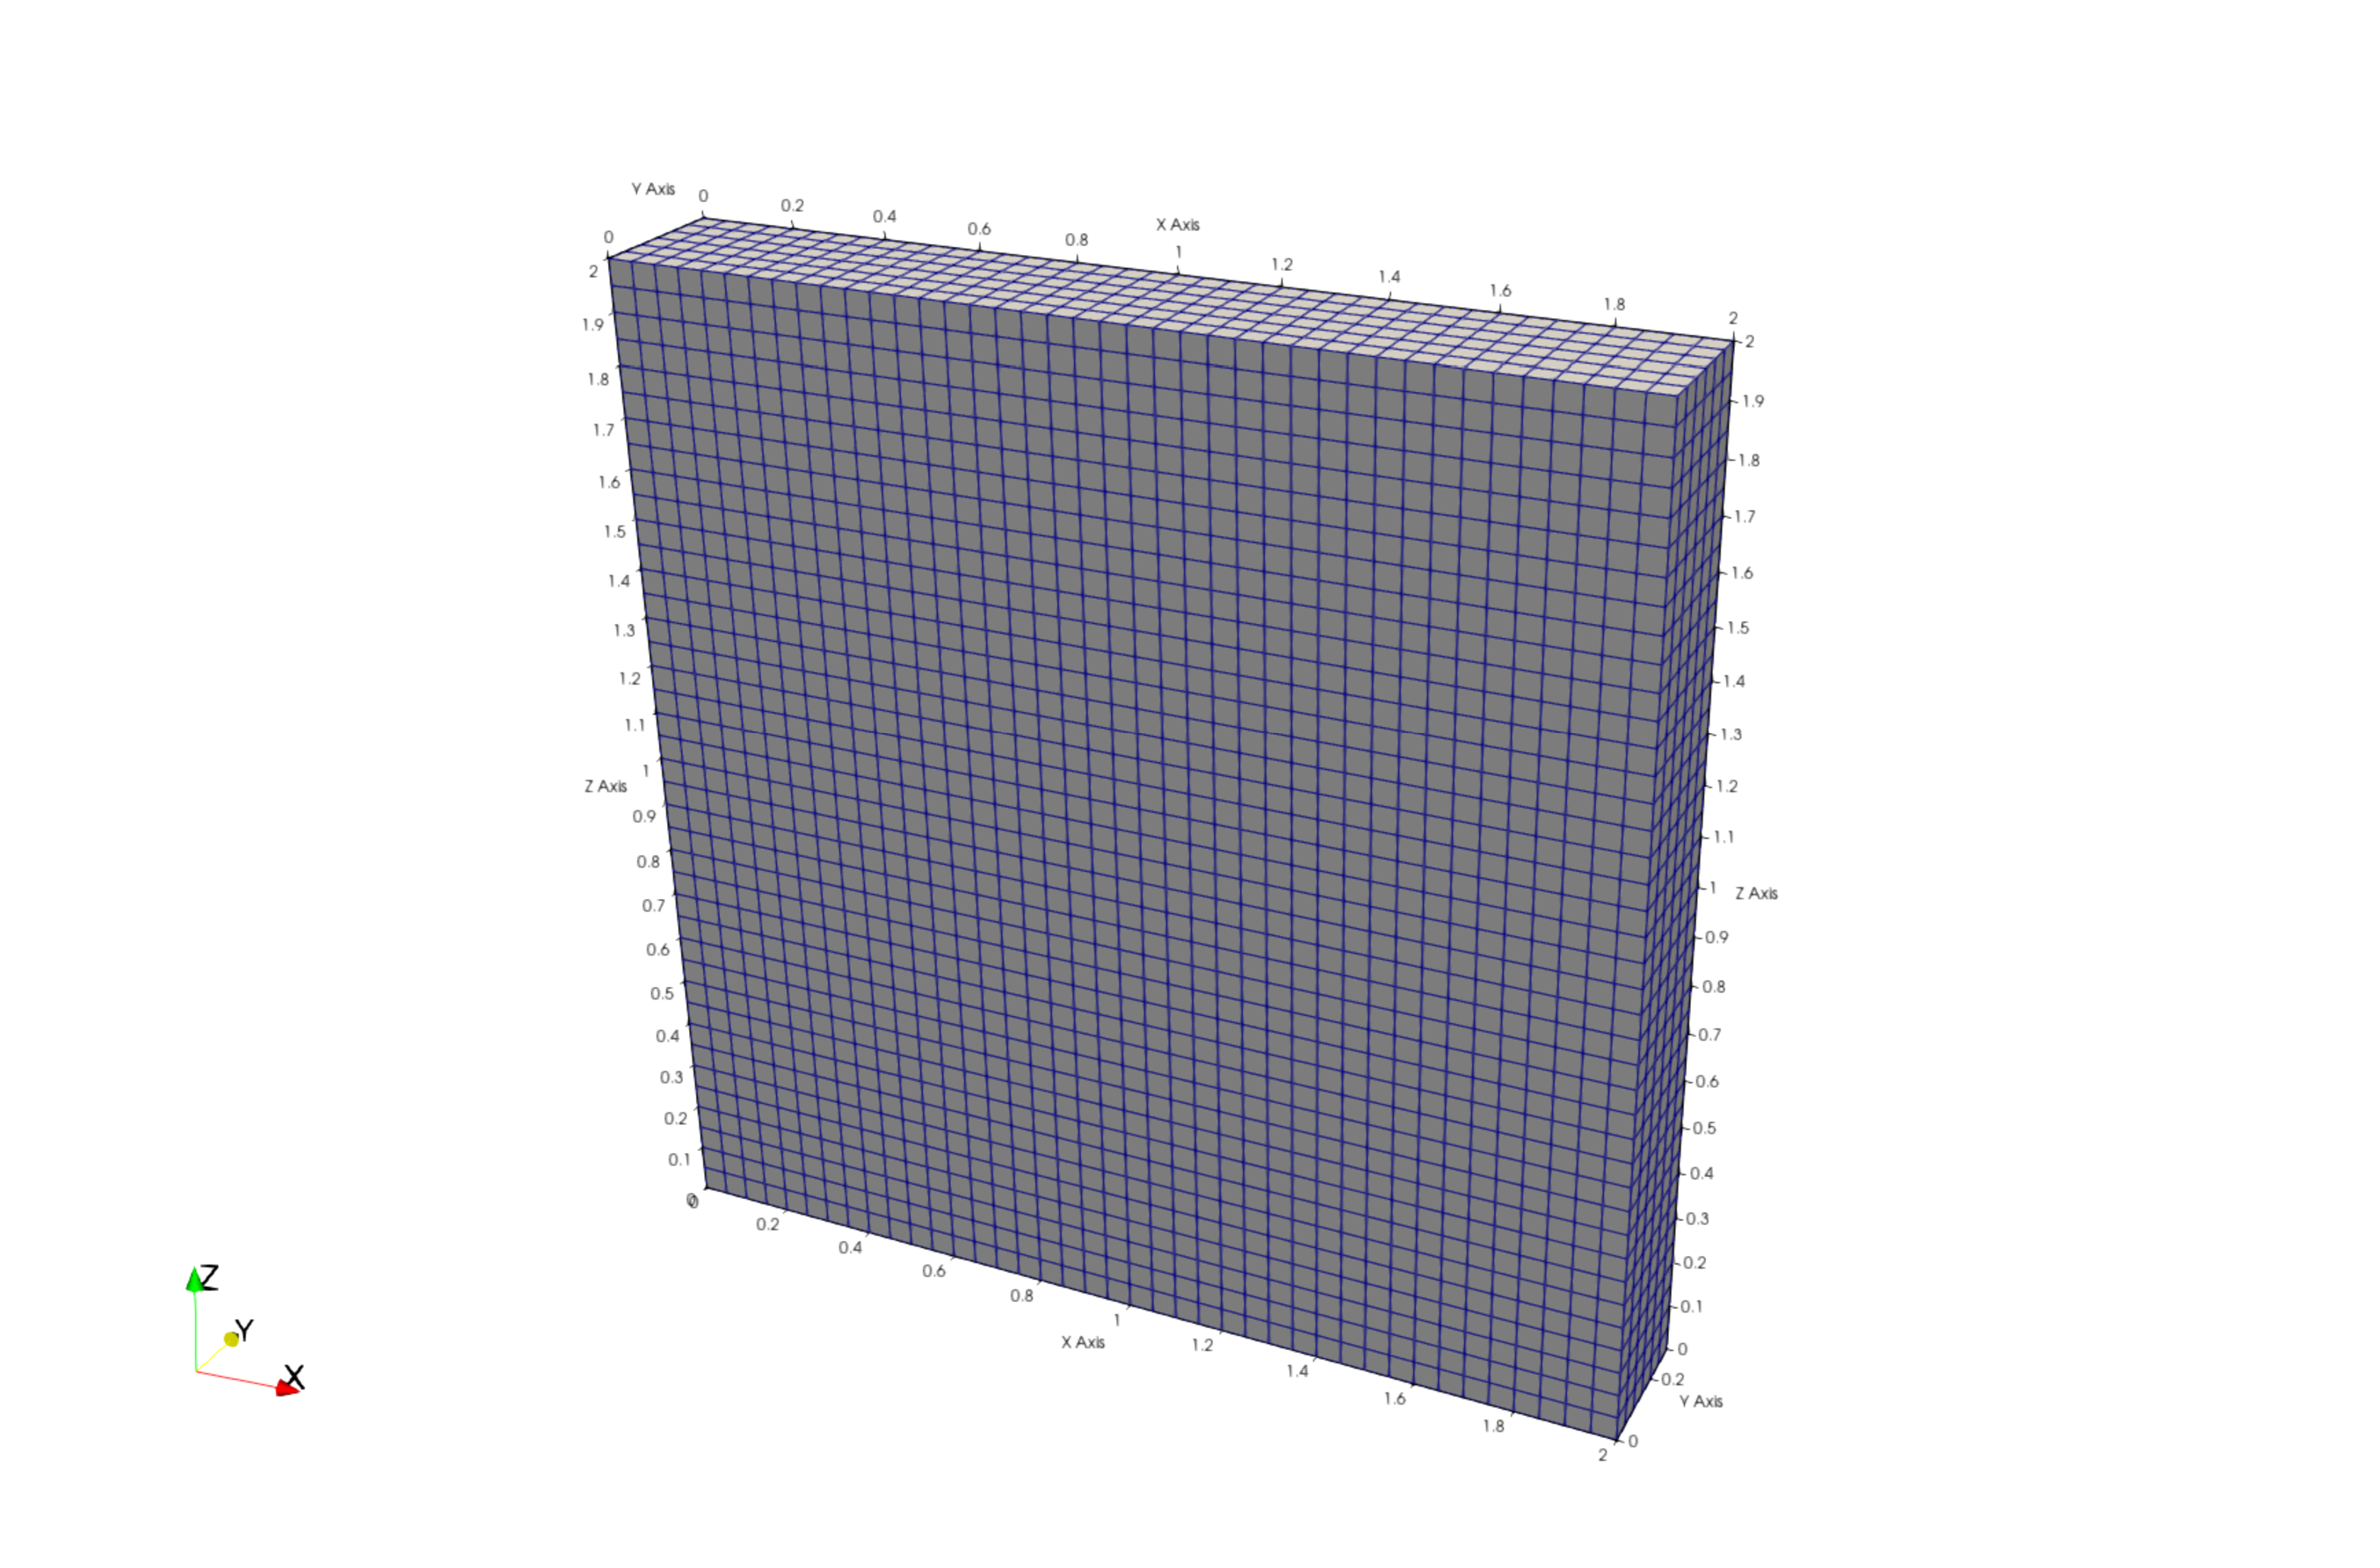
\includegraphics[width=18truecm]{pics/3d-dambreak/mesh.pdf}
	\caption{メッシュ}
	\label{fig:3d-dambreak-mesh}
\end{figure}

\begin{figure}[htbp]
	\centering
	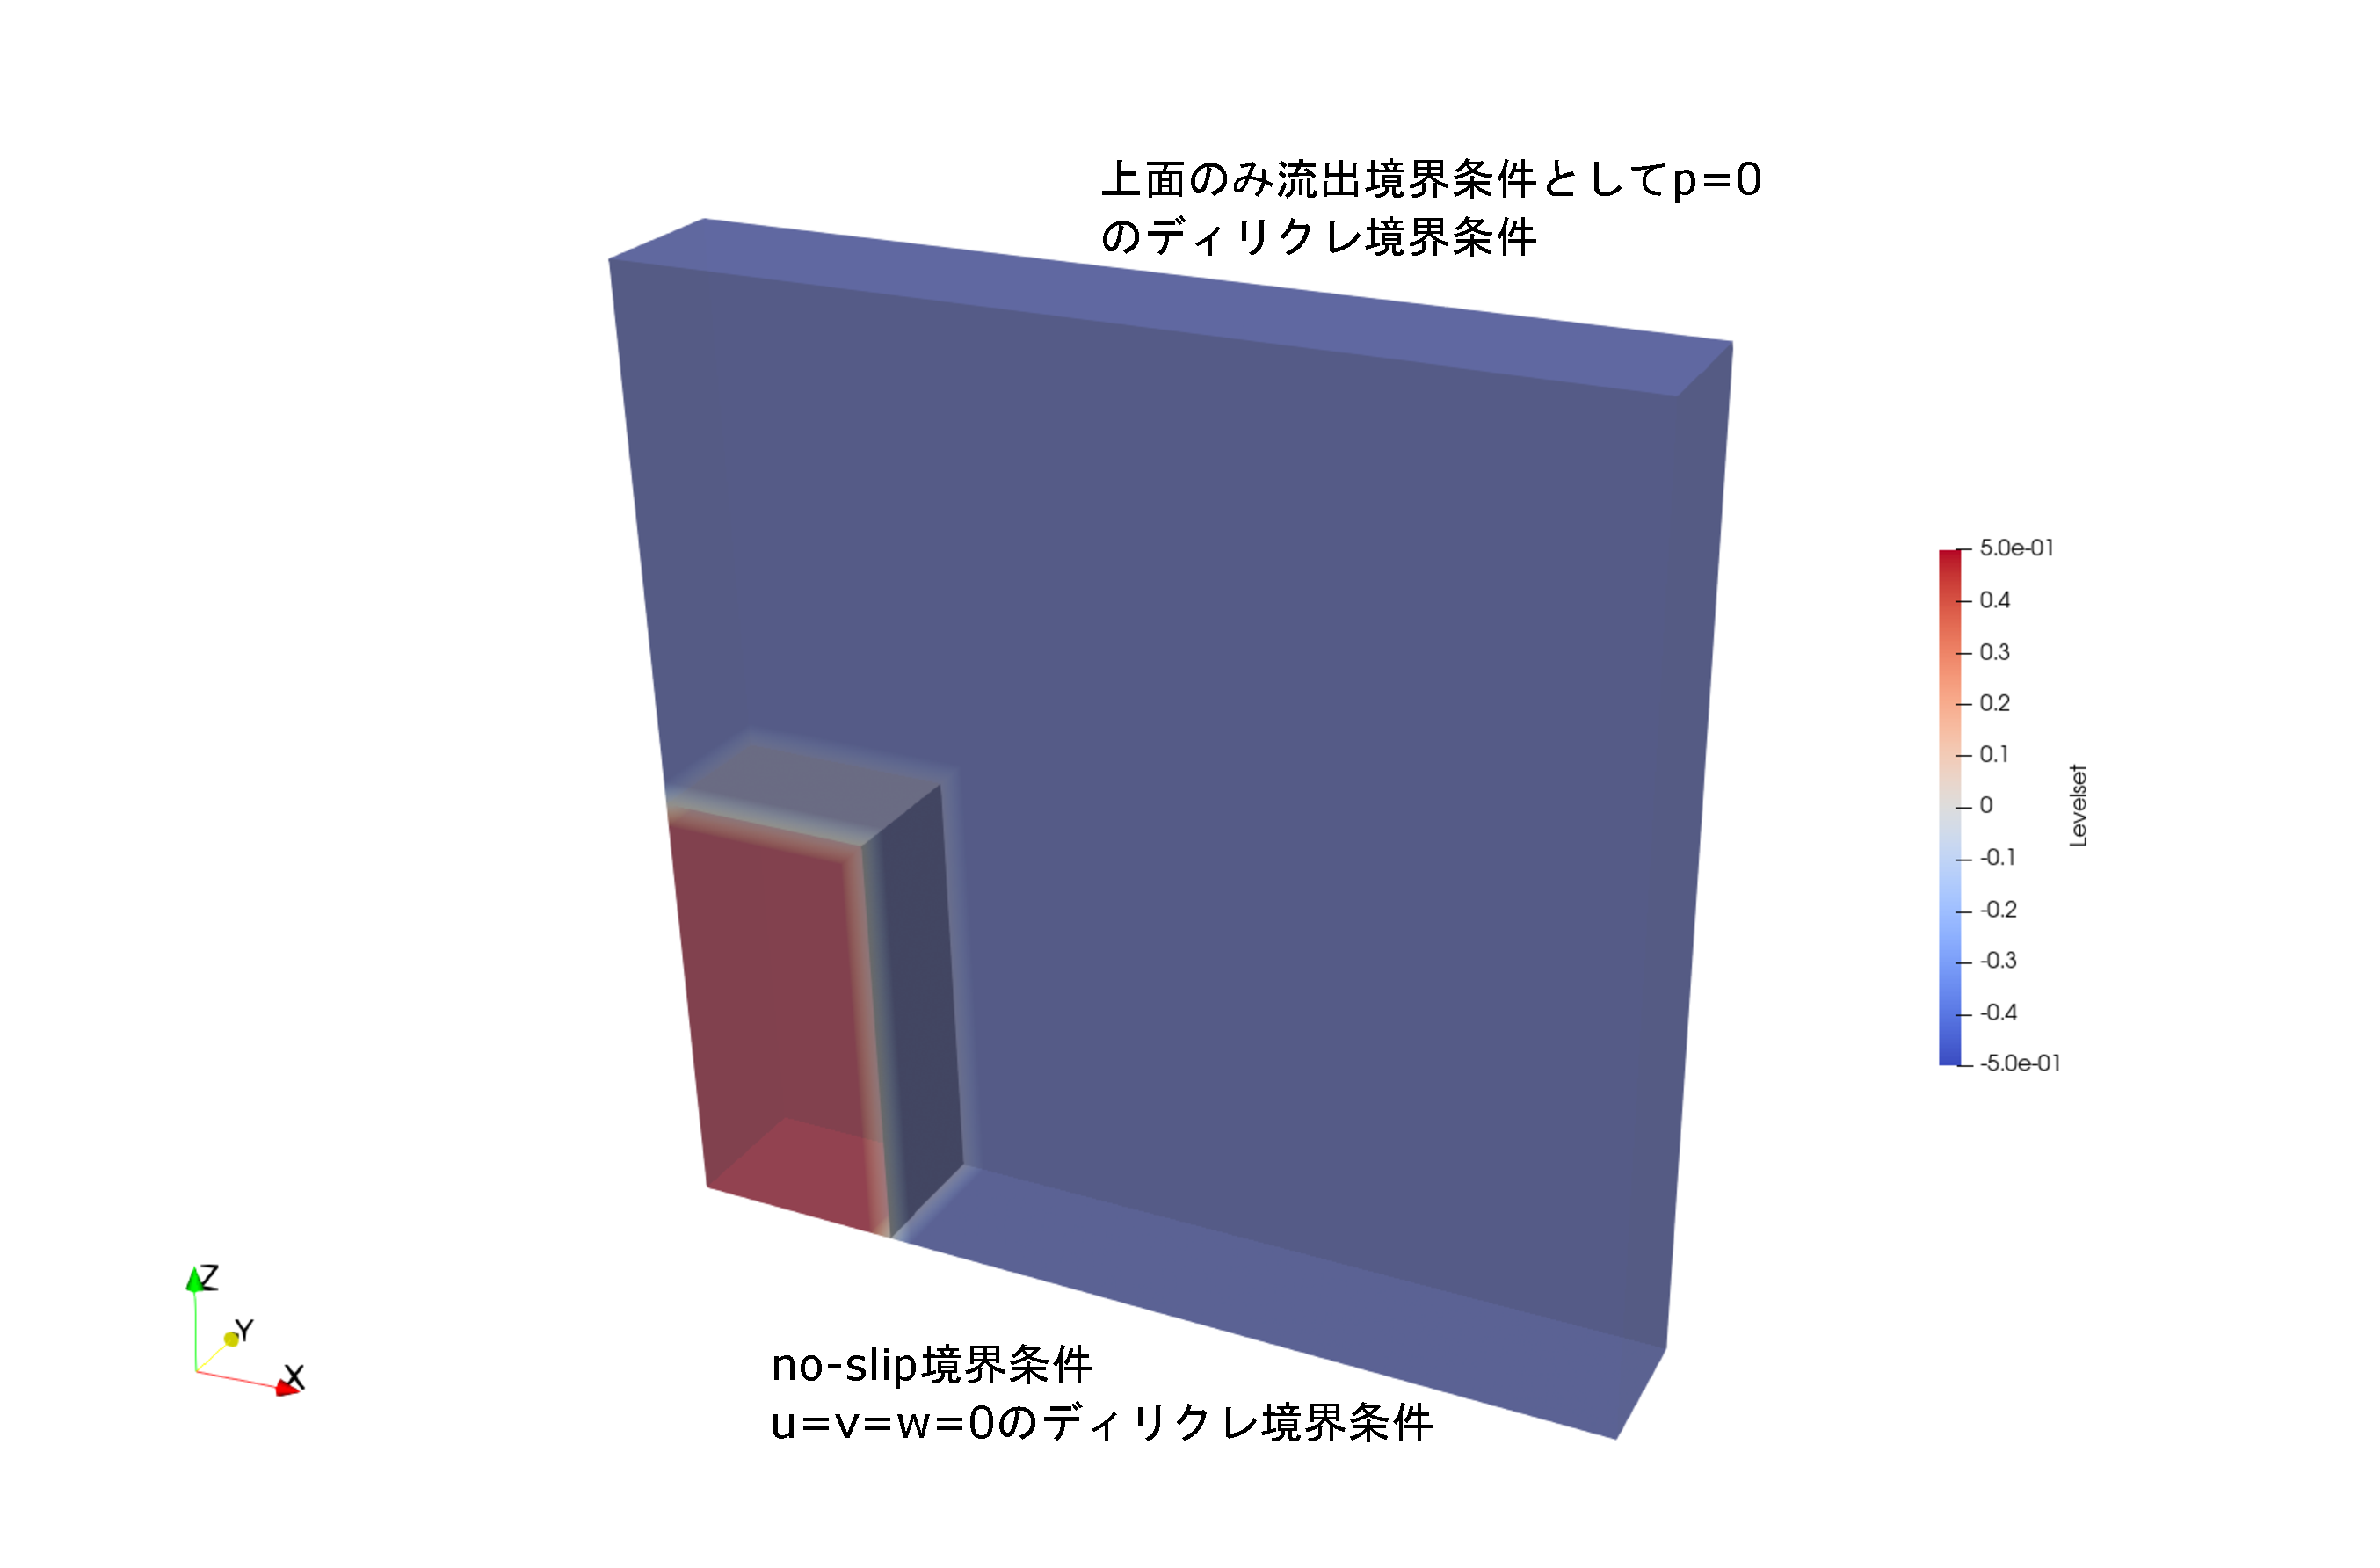
\includegraphics[width=18truecm]{pics/3d-dambreak/levelset_init.pdf}
	\caption{初期のレベルセット関数}
	\label{fig:3d-dambreak-mesh}
\end{figure}

\subsection{解析結果}

物性値Case$1$の水と空気の物性値のオーダーでは計算が発散してしまう。解析パラメータ$1$, $2$でも同様に発散する。
物性値Case$2$の水と空気(の密度と粘性係数が10倍)の物性値のオーダーでは、解析パラメータ$1$では発散し、$2$でヘビサイド関数の$D$を大きく取ることで安定化した。

\begin{figure}[htbp]
	\centering
	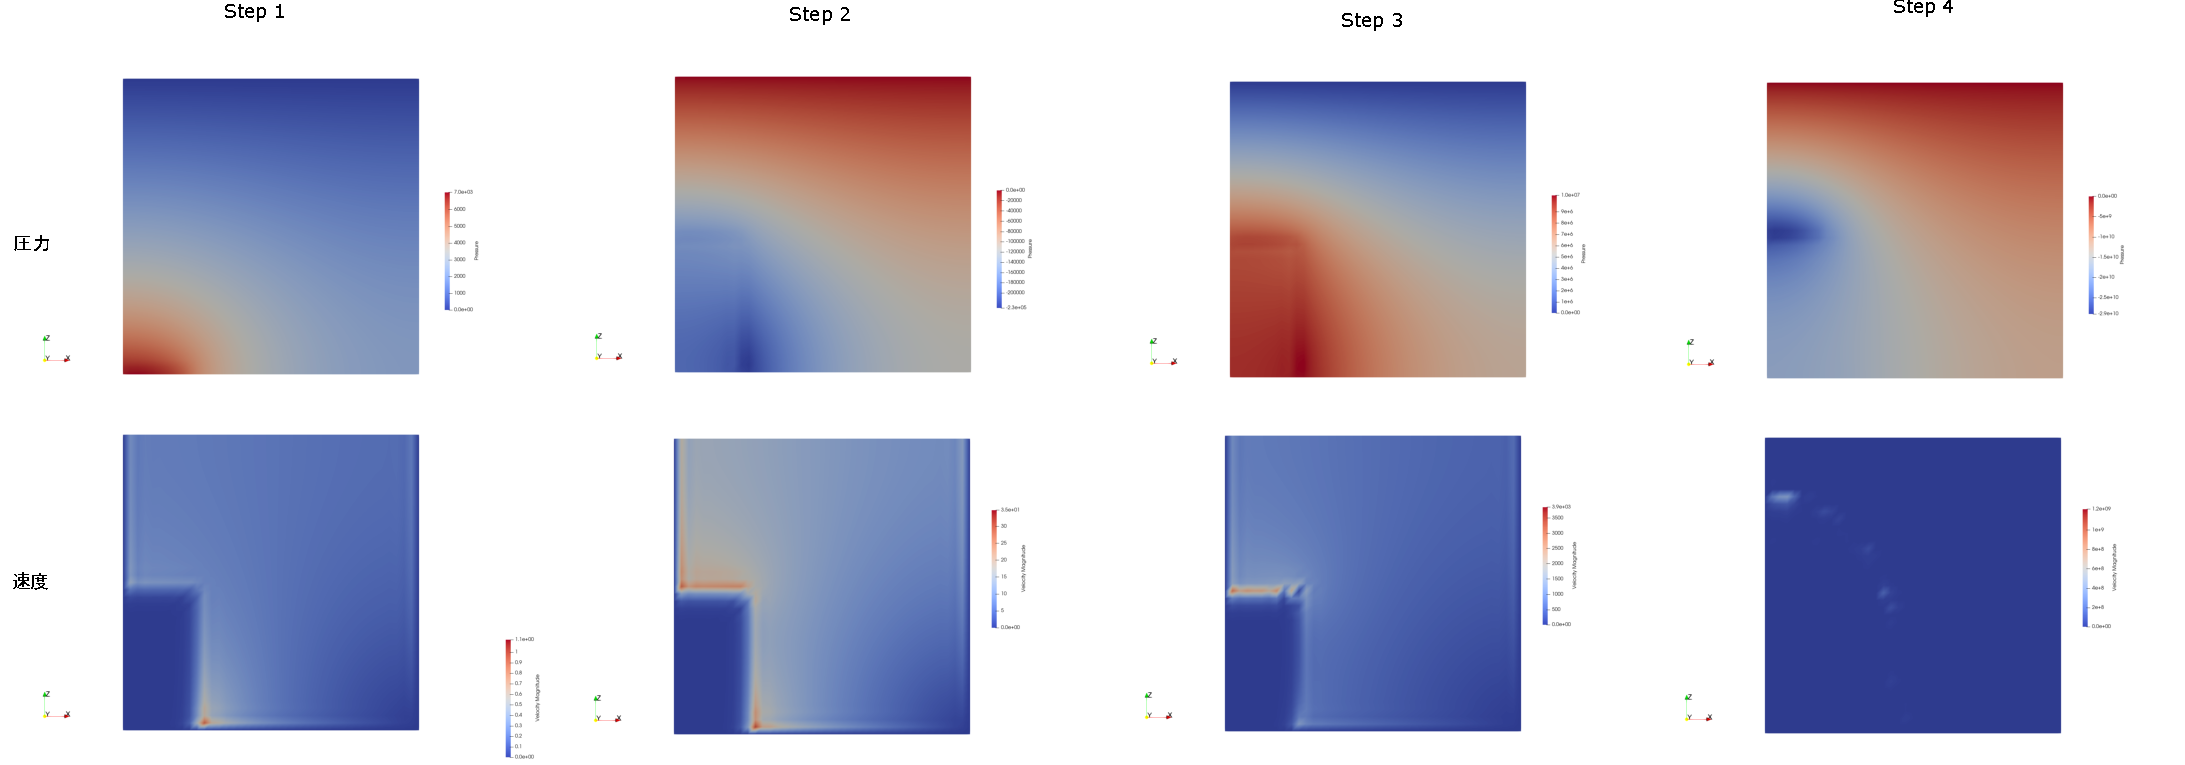
\includegraphics[width=18truecm]{pics/3d-dambreak/diverge_water_air.pdf}
	\caption{物性値がCase1の差が大きい場合の初期の発散する様子。圧力が振動している。}
	\label{fig:3d-dambreak-diverge}
\end{figure}

\begin{figure}[htbp]
	\centering
	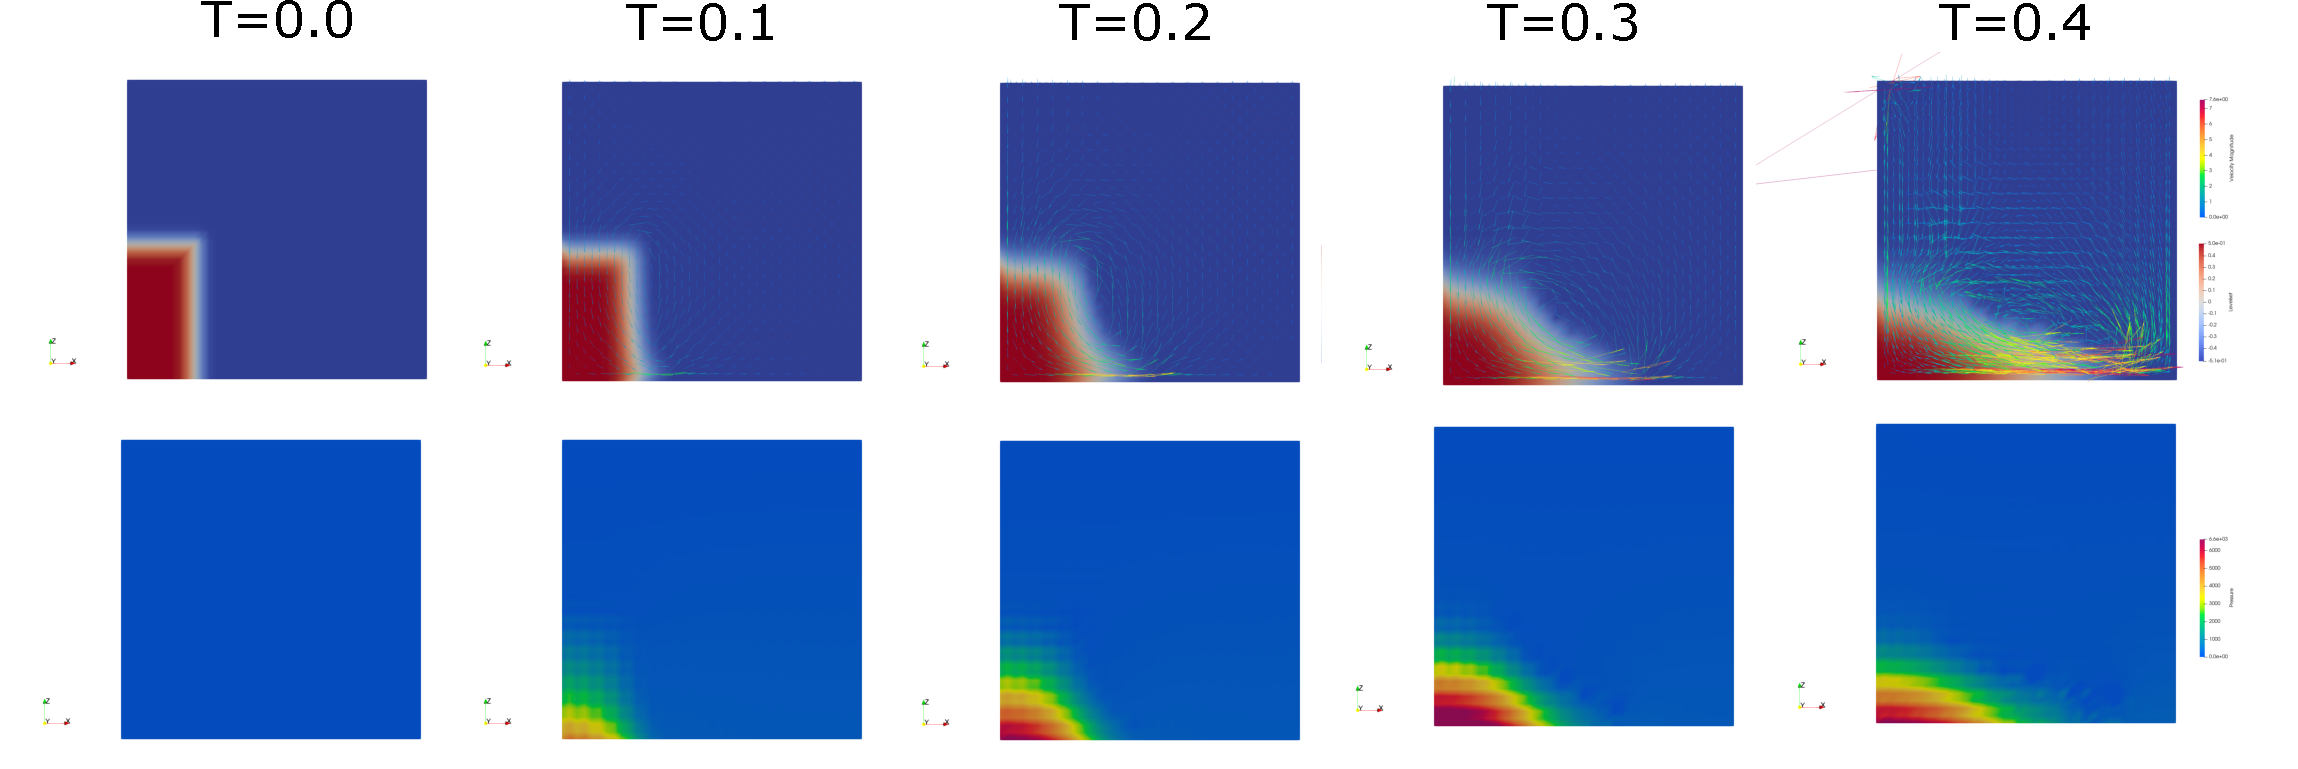
\includegraphics[width=18truecm]{pics/3d-dambreak/levelset_velocity.pdf}
	\caption{物性値がCase2の差が小さい場合の結果。ヘビサイド関数Dの値を大きくすることで安定に計算できた。}
	\label{fig:3d-dambreak-diverge}
\end{figure}

\newpage
\section{3次元のバブル流れ問題}
\subsection{解析条件}

\renewcommand{\arraystretch}{1}
\begin{table}[H]
	\centering
	\caption{解析パラメータ}
	\begin{tabular}{ccccccc}
		\hline
		Test case & $\rho_1$ & $\rho_2$ & $\mu_1$ & $\mu_2$ & $\mathrm{g}$ & $\sigma$\\
		\hline 
		Case$1$ & $1000$ & $100$ & $10$ & $1$   & $0.98$ & $24.5$ \\
		Case$2$ & $1000$ & $1$   & $10$ & $0.1$ & $0.98$ & $1.96$ \\
		\hline         
	\end{tabular}
	\label{table:mars-env}
\end{table}
\renewcommand{\arraystretch}{1.0}

\renewcommand{\arraystretch}{1}
\begin{table}[H]
	\centering
	\caption{解析パラメータ}
	\begin{tabular}{ccc}
		\hline
		Test case & メッシュ幅$dx$ & ヘビサイド関数パラメータ$D$\\
		\hline 
		Case$1$ & $0.05$ & $0.05$\\
		\hline         
	\end{tabular}
	\label{table:mars-env}
\end{table}
\renewcommand{\arraystretch}{1.0}

\begin{figure}[htbp]
	\centering
	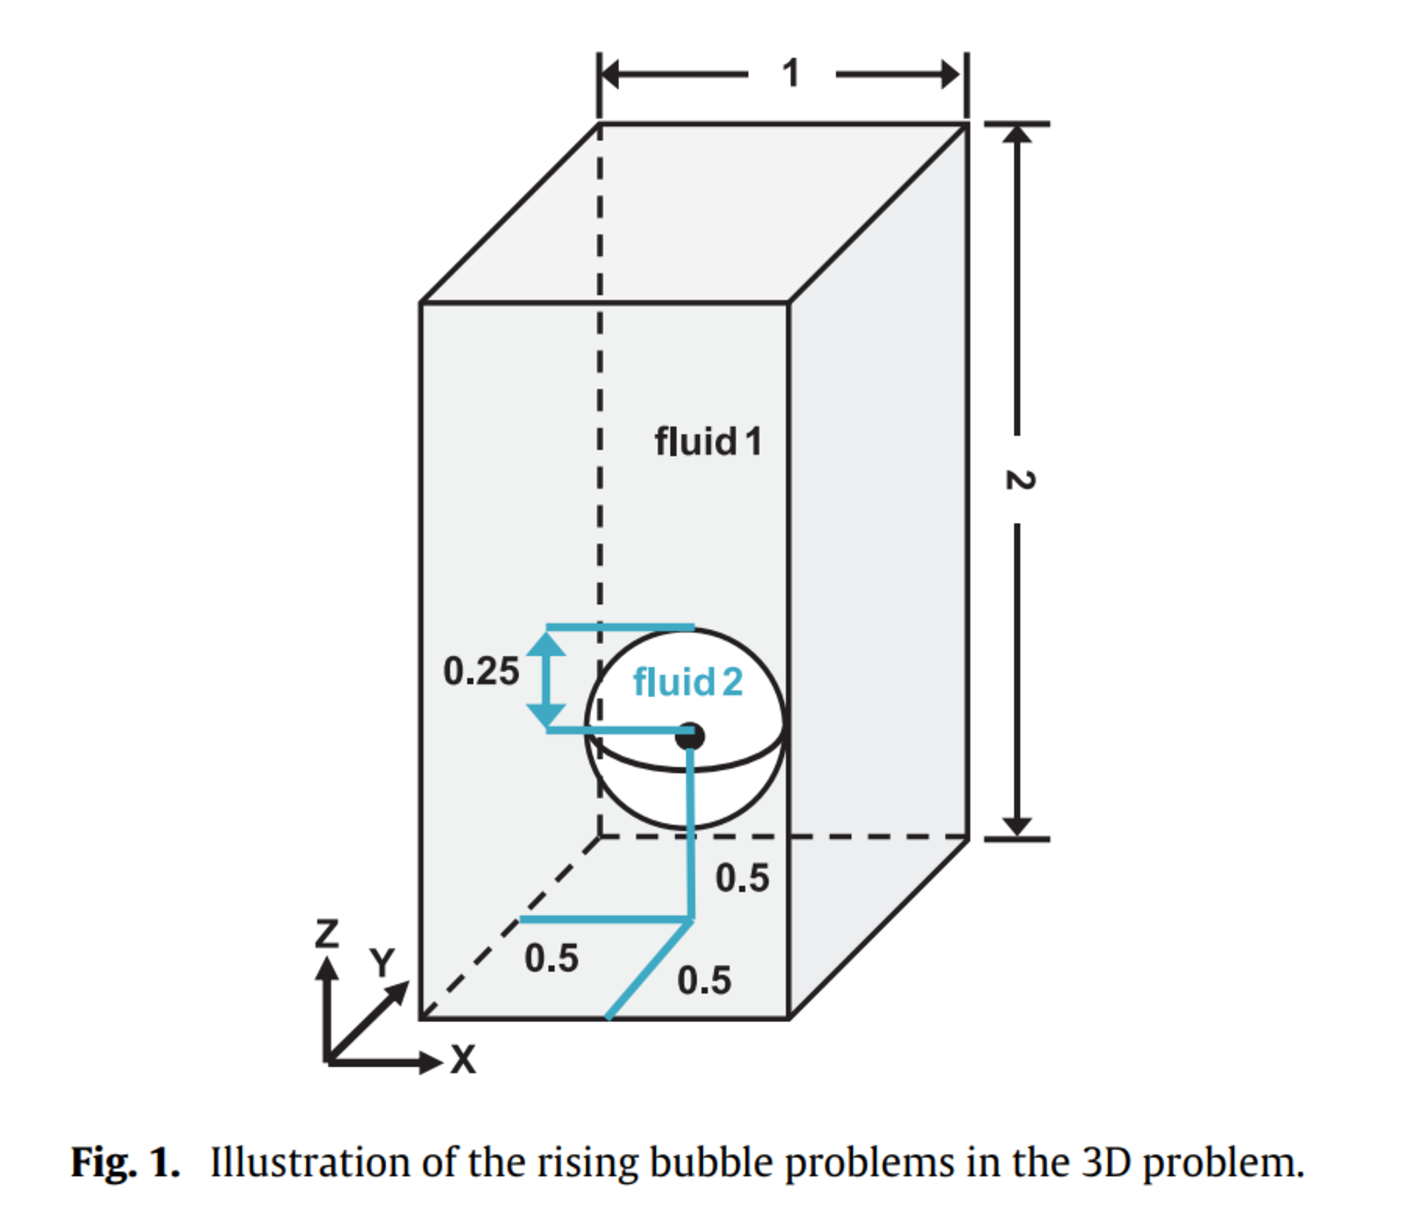
\includegraphics[width=10truecm]{pics/3d-bubble/setting.pdf}
	\caption{解析条件~\cite{Safi2017}}
	\label{fig:3d-bubble-setting}
\end{figure}

\begin{figure}[htbp]
	\centering
	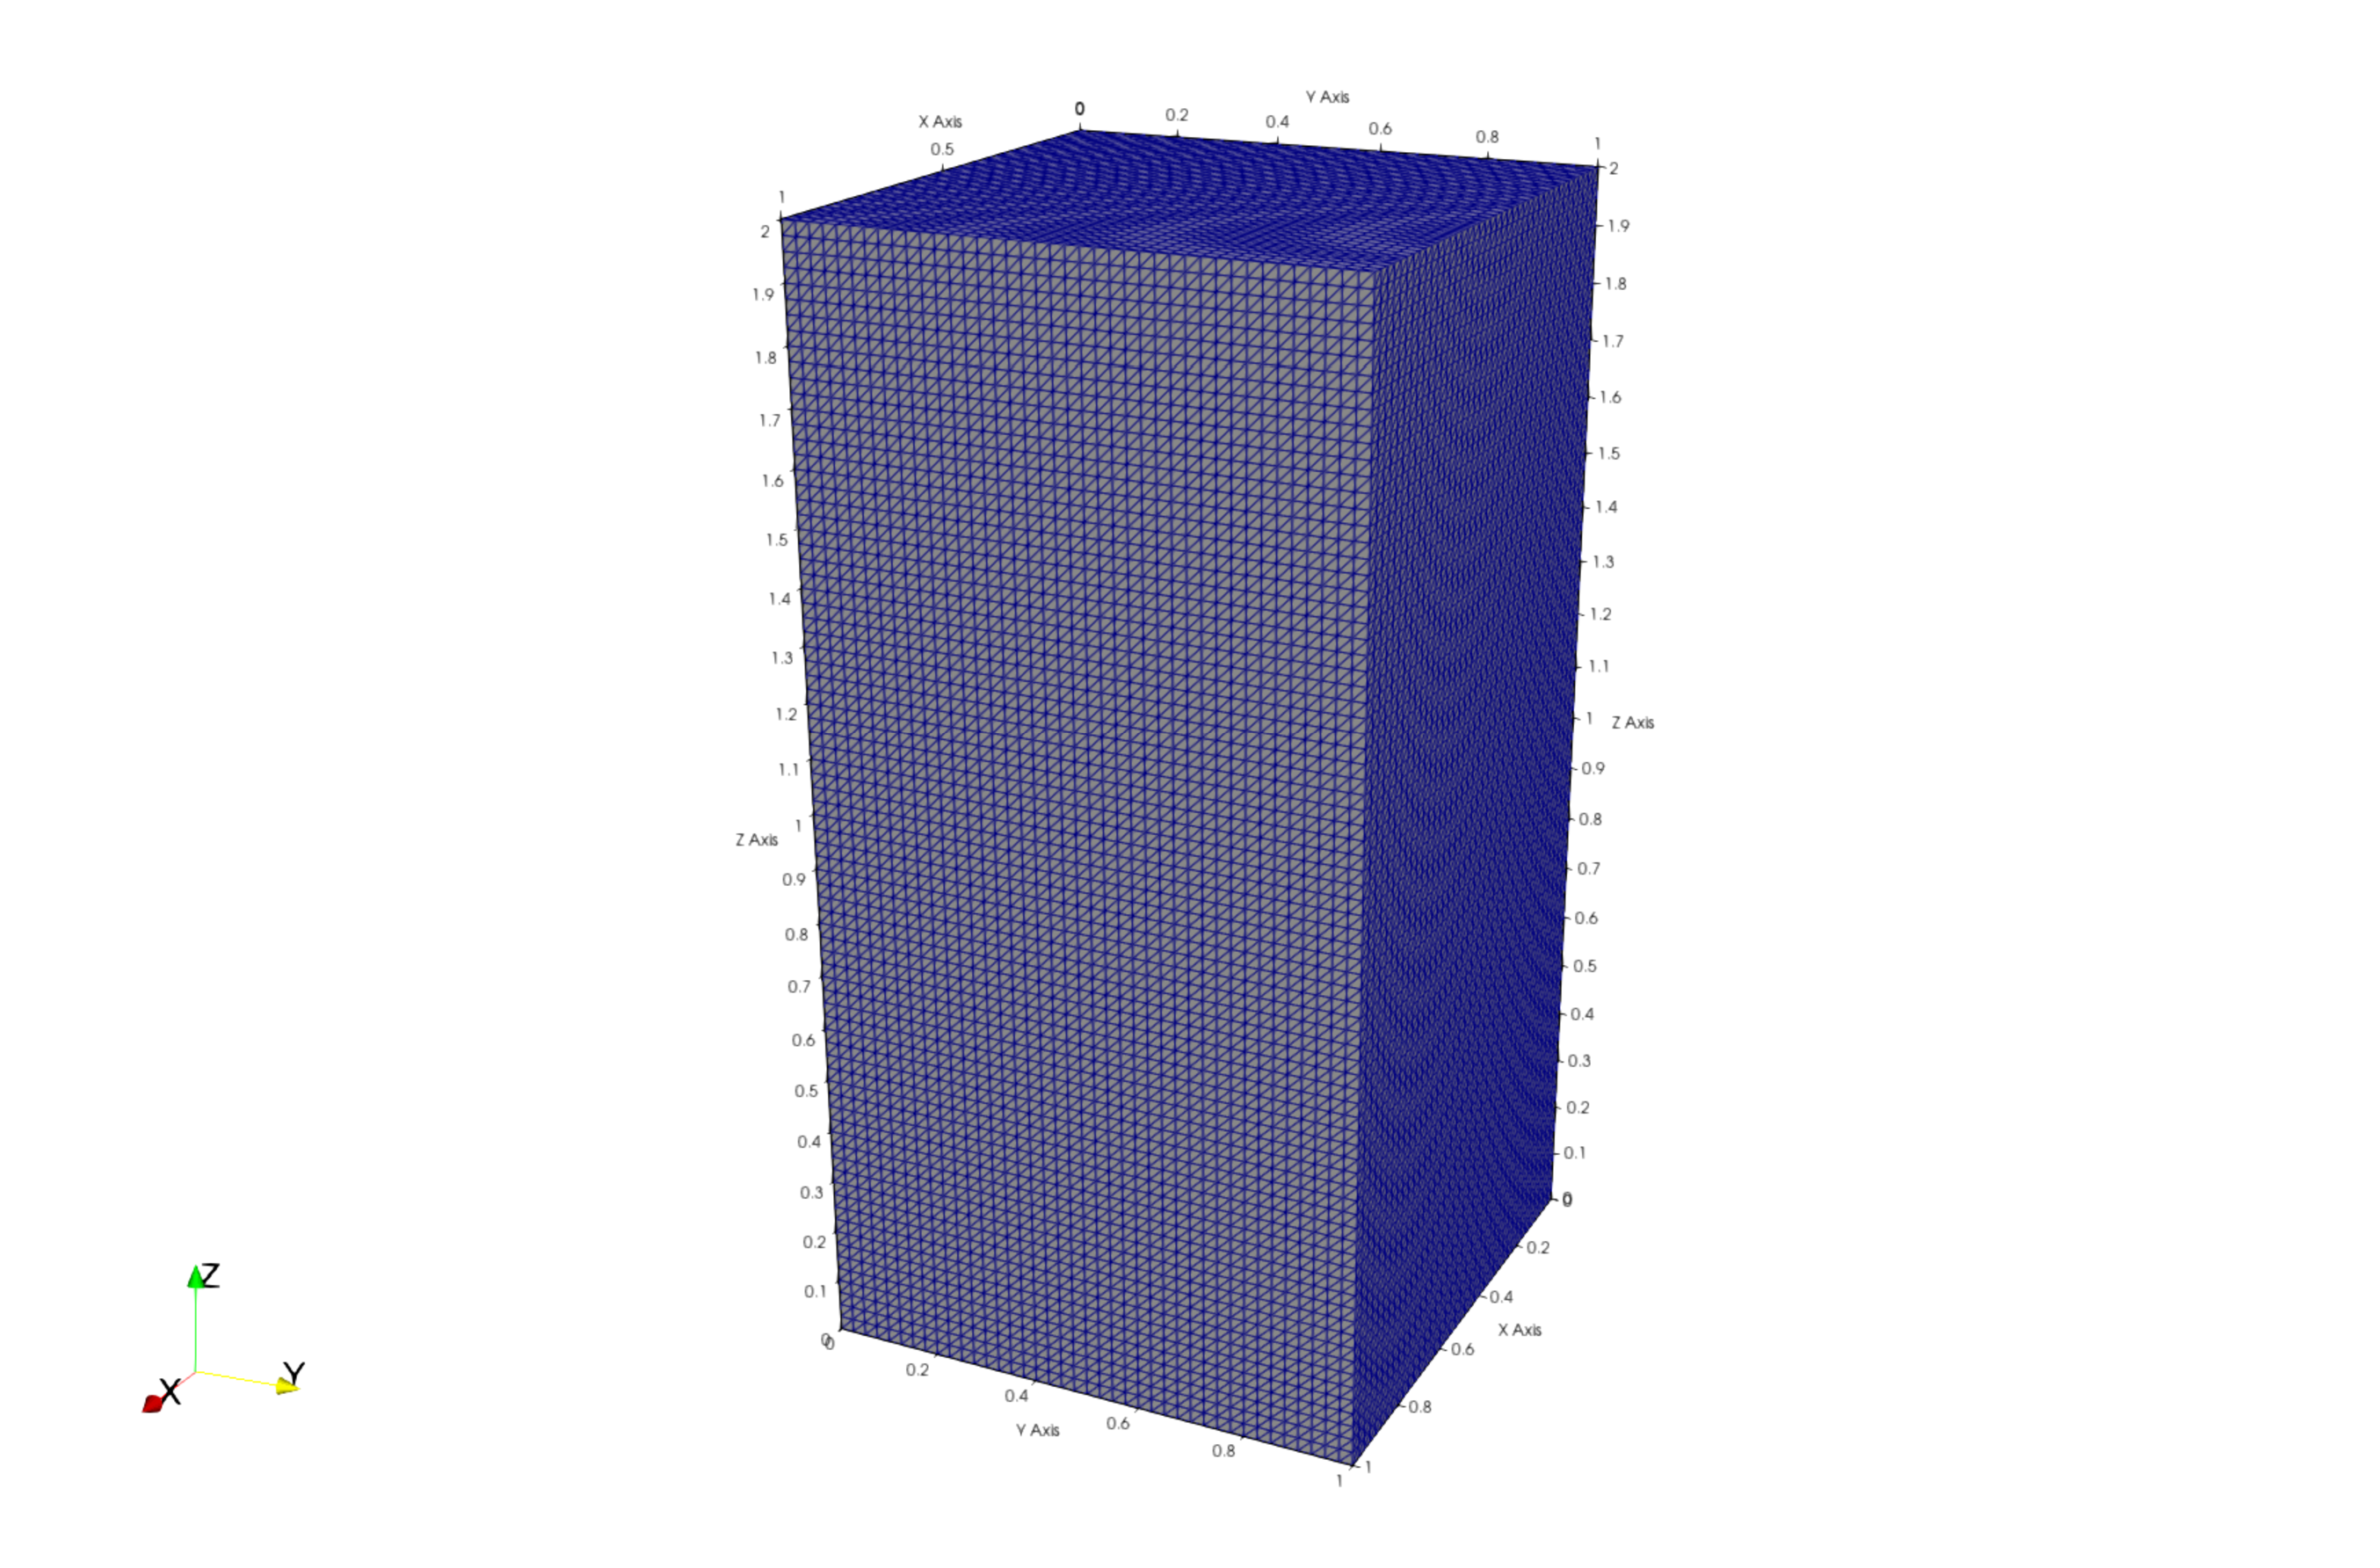
\includegraphics[width=10truecm]{pics/3d-bubble/mesh.pdf}
	\caption{メッシュ}
	\label{fig:3d-bubble-mesh}
\end{figure}

\begin{figure}[htbp]
	\centering
	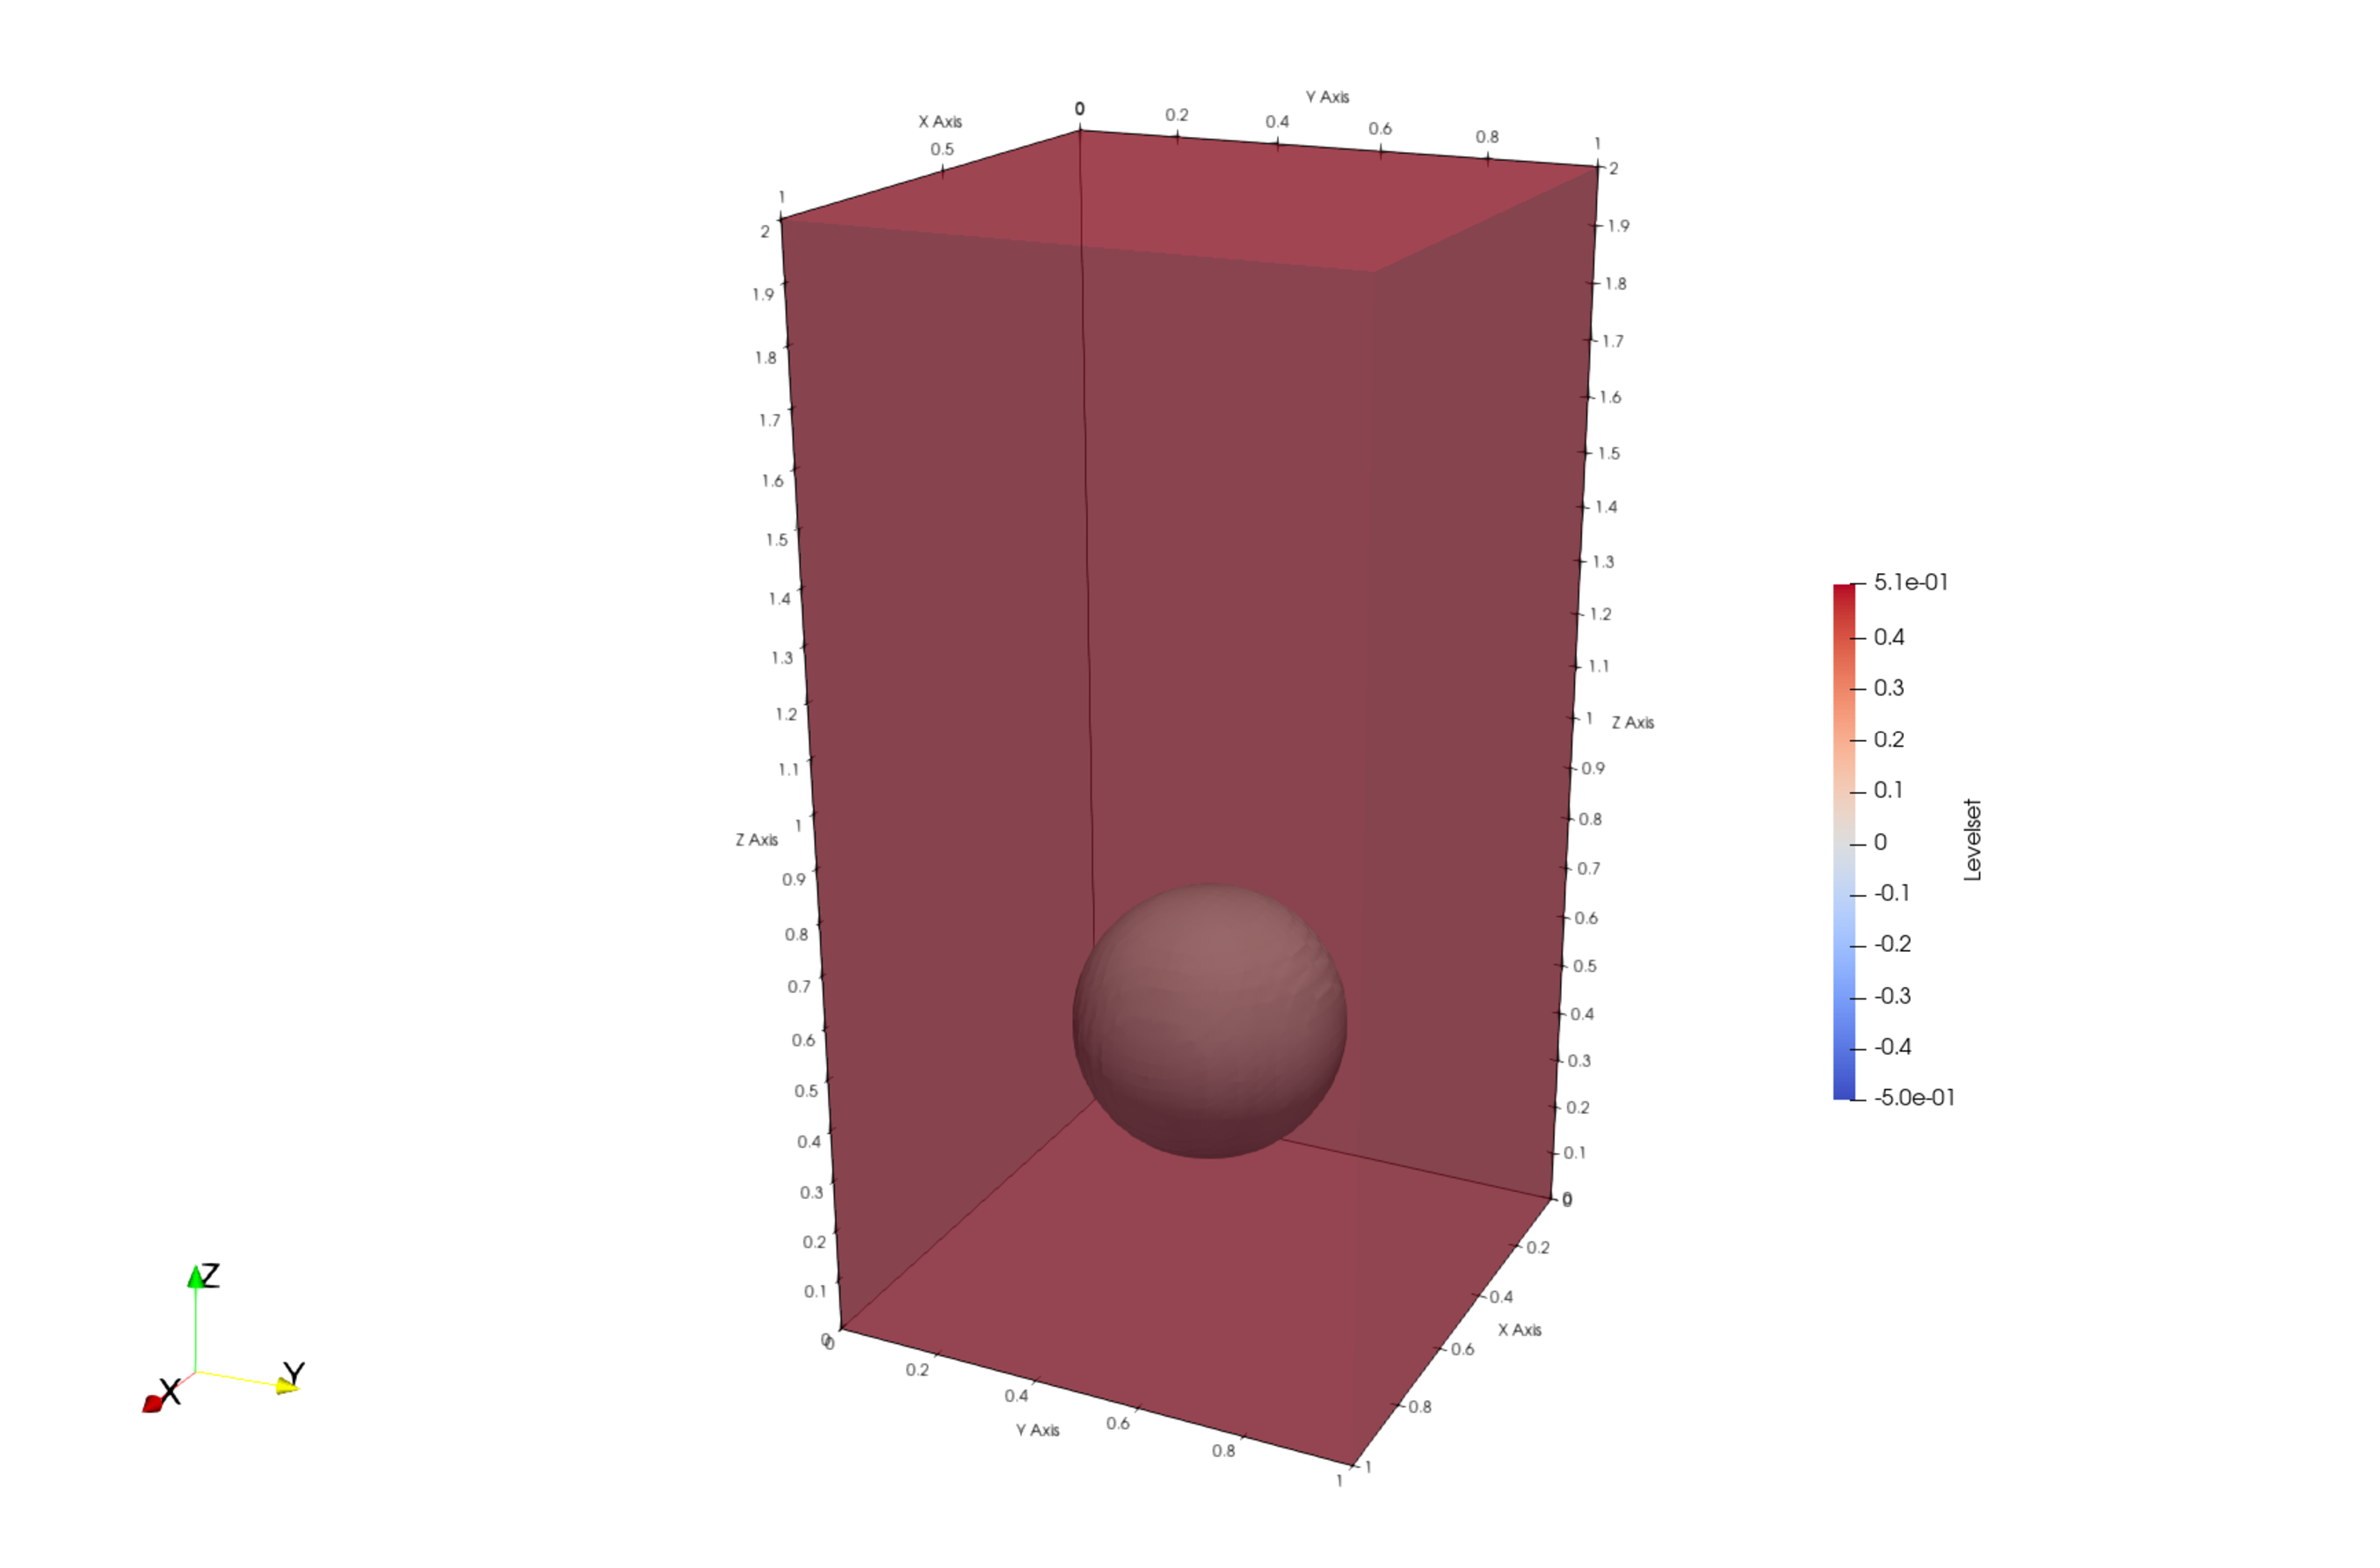
\includegraphics[width=10truecm]{pics/3d-bubble/levelset_t0_3d.pdf}
	\caption{初期状態のレベルセット関数}
	\label{fig:3d-bubble-levelset_t0_3d}
\end{figure}


\subsection{解析結果}

\begin{figure}[htbp]
	\centering
	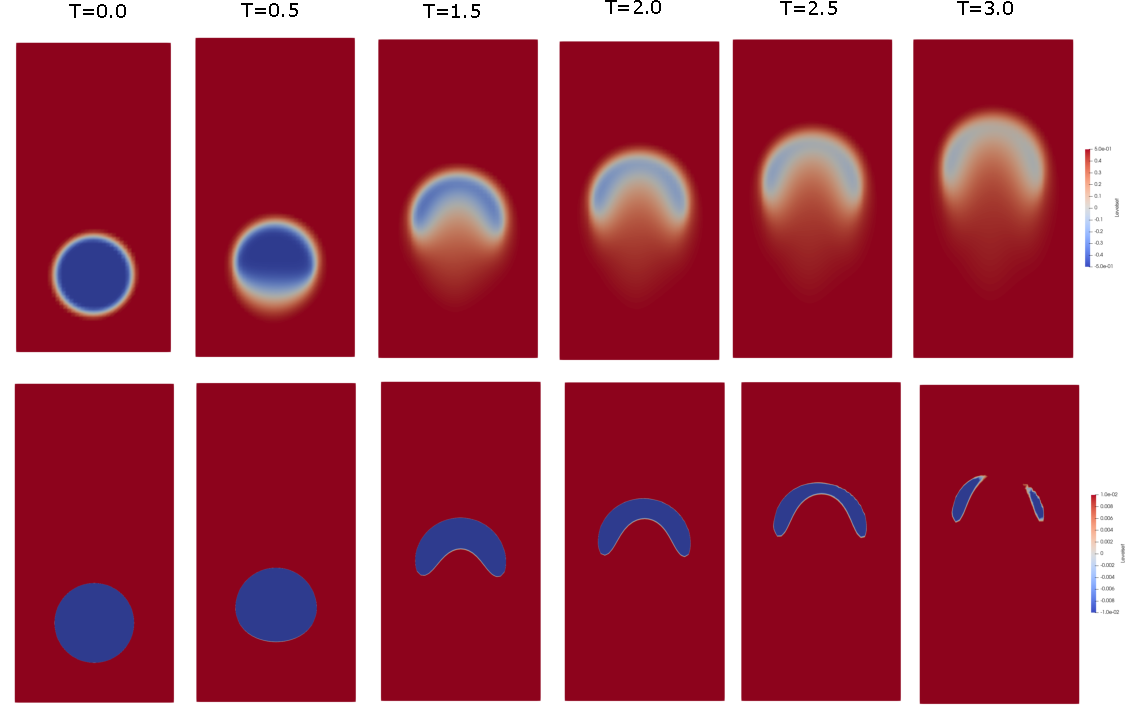
\includegraphics[width=18truecm]{pics/3d-bubble/levelset_t0-3.pdf}
	\caption{結果 表面張力なし}
	\label{fig:3d-bubble-levelset_t0-3}
\end{figure}

\begin{figure}[htbp]
	\centering
	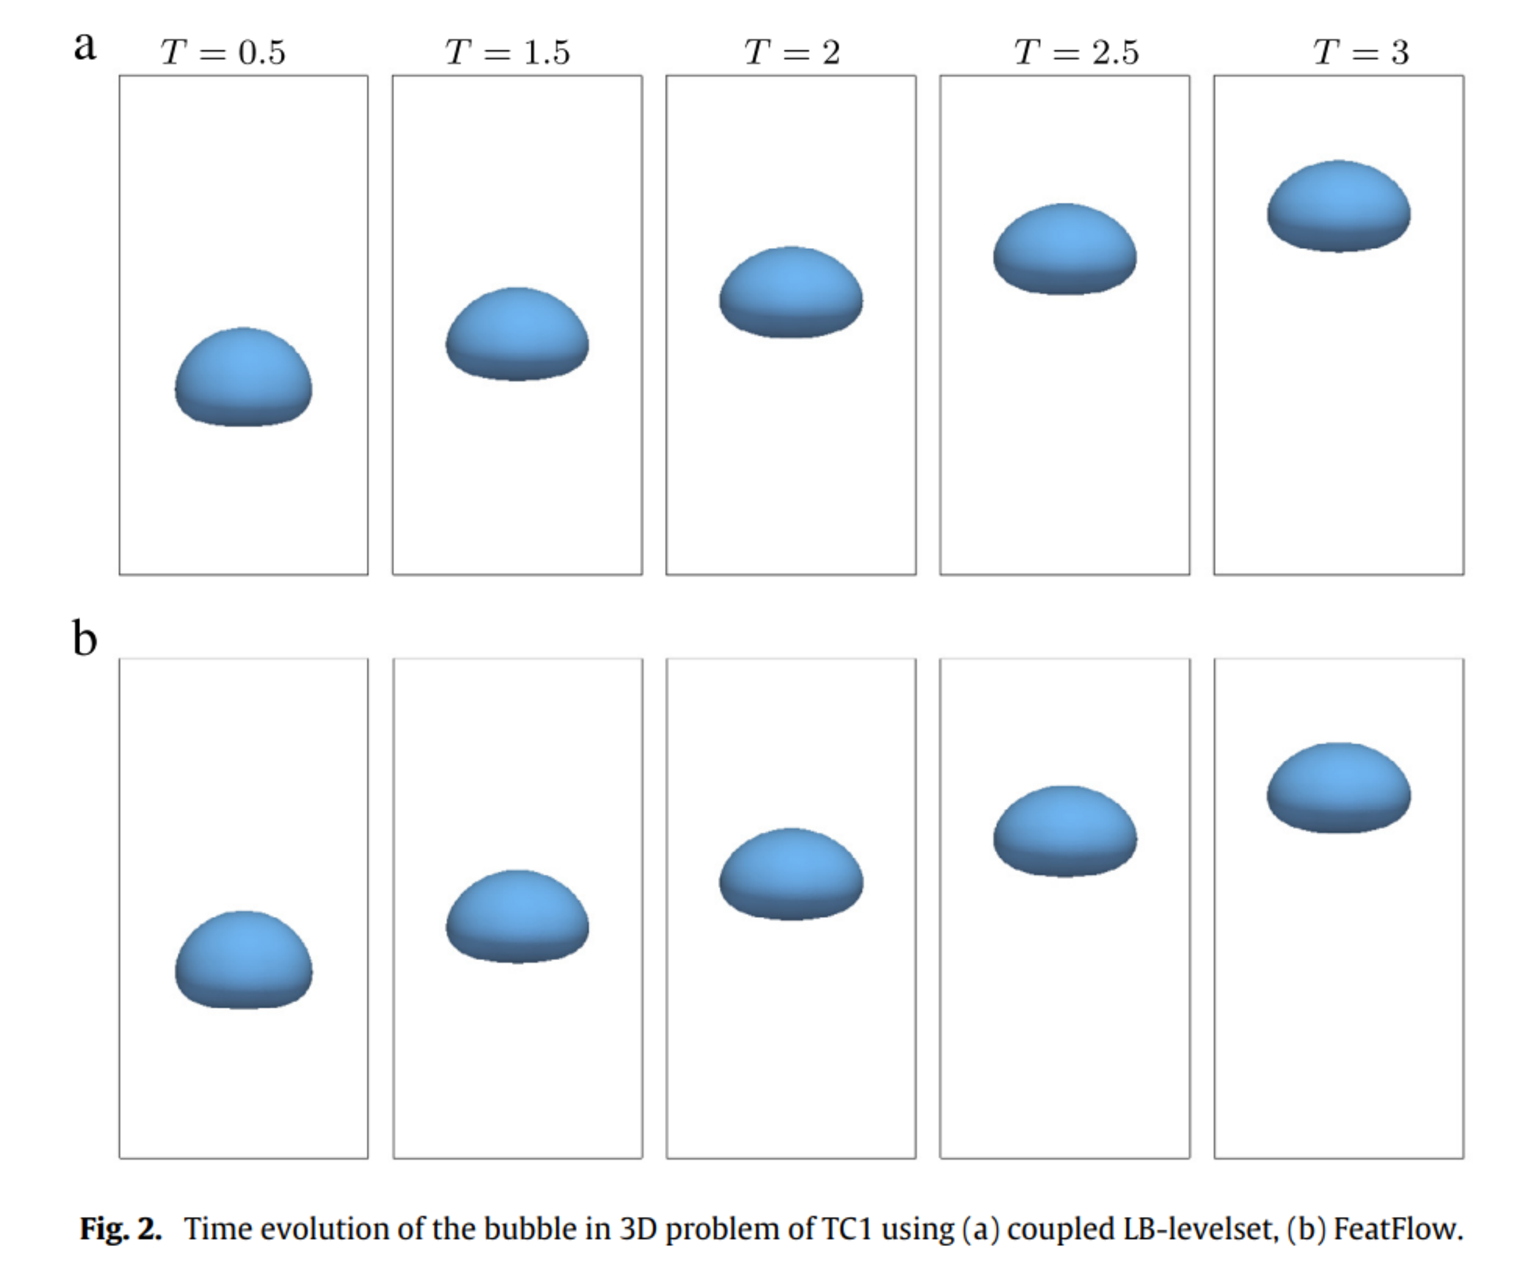
\includegraphics[width=10truecm]{pics/3d-bubble/result-ref.pdf}
	\caption{参考文献結果~\cite{Safi2017}}
	\label{fig:3d-bubble-result-ref}
\end{figure}

\begin{thebibliography}{99}
	\bibitem{Safi2017} Safi, M. A., Prasianakis, N. \& Turek, S. Benchmark computations for 3D two-phase flows: A coupled lattice Boltzmann-level set study. Comput. Math. Appl. 73, 520–536 (2017)
\end{thebibliography}
\end{document}

